\documentclass[border=10pt,tikz]{standalone}
\usepackage{tikz}
\usetikzlibrary{positioning,arrows.meta,shapes}
\begin{document}
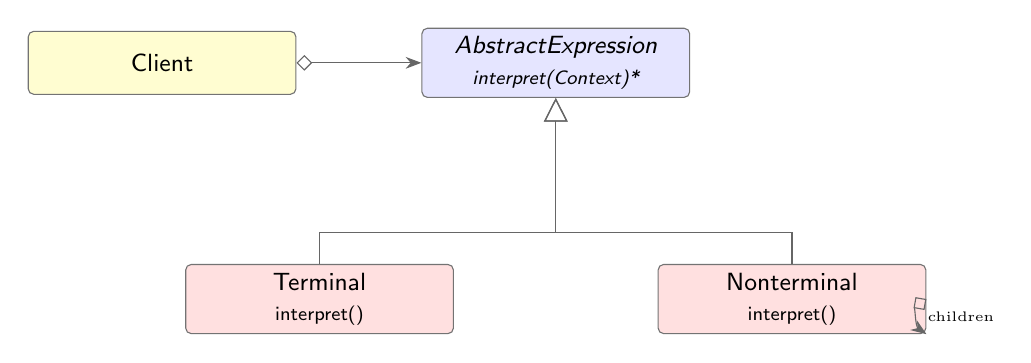
\begin{tikzpicture}[
  font=\sffamily\small,
  cls/.style={rectangle, rounded corners=2pt, draw=black!55, line width=0.4pt,
              minimum height=8mm, minimum width=34mm, inner sep=3pt, fill=white, align=center},
  abs/.style={cls, fill=blue!10, font=\sffamily\itshape\small},
  con/.style={cls, fill=red!12},
  cli/.style={cls, fill=yellow!18},
  inh/.style={-{Triangle[length=3mm,width=3mm,open]}, draw=black!60, line width=0.45pt},
  agg/.style={{Diamond[length=2mm,width=2mm,open]}-{Stealth[length=2mm]}, draw=black!60}
]
\node[cli] (c)   at (-5, 1) {Client};
\node[abs] (e)   at ( 0, 1) {AbstractExpression \\ \scriptsize interpret(Context)*};
\node[con] (te)  at (-3,-2) {Terminal \\ \scriptsize interpret()};
\node[con] (nt)  at ( 3,-2) {Nonterminal \\ \scriptsize interpret()};

\draw[agg] (c.east) -- (e.west);
\draw[inh] (te.north) -- ++(0,0.4) -| (e.south);
\draw[inh] (nt.north) -- ++(0,0.4) -| (e.south);
\draw[agg] (nt.east) to[bend right=55] node[right, font=\tiny]{children} (nt.south east);
\end{tikzpicture}
\end{document}
